\documentclass[11pt]{article}
\usepackage[T1]{fontenc}
\usepackage[utf8]{inputenc}
\usepackage[
    left=1in,
    right=1in,
    top=0.6in,
    bottom=1in
]{geometry}

\usepackage{amsmath,amssymb}
\usepackage{graphicx}
\usepackage{booktabs}
\usepackage{float}
\usepackage[hidelinks]{hyperref}
\usepackage{tabularx}
\usepackage{caption}
\usepackage{tikz}
\usetikzlibrary{arrows.meta, positioning}
\usepackage{pgfplots}
\pgfplotsset{compat=1.18}
\setlength{\emergencystretch}{3em}


% Latency chart colours, light to dark, and the UR setting in grey.
\definecolor{latA}{HTML}{A9CDD8}
\definecolor{latB}{HTML}{6FA5B5}
\definecolor{latC}{HTML}{3A7C96}
\definecolor{latD}{HTML}{1E4A66}
\definecolor{latE}{HTML}{BDBDBD}

% File links point to the GitLab repository, branch teleop-refactor.

\title{Week 6 \& 7 Status Report}
\author{Yiran Liu, To: Dr.Pengcheng Xi}
\date{\today}

\begin{document}
\maketitle

\noindent
Most of the progress has been reported verbally, this document extends on the details. File names are all clickable and linked to repository.

\section{Teleoperation Refactor}

Three of the five stages are complete and the fourth is designed.
The design is \href{https://gitlabc.nrc-cnrc.gc.ca/Yiran.Liu/nrc_robot_manipulation/-/blob/teleop-refactor/Documentation/Journal/2026Sep/TeleopRefactor.md}{\texttt{TeleopRefactor.md}}; daily progress is on
\href{https://gitlabc.nrc-cnrc.gc.ca/Yiran.Liu/nrc_robot_manipulation/-/blob/teleop-refactor/Documentation/Journal/2026Oct/TeleopRefactorTaskPanel.md}{\texttt{TeleopRefactorTaskPanel.md}}.

\begin{table}[H]
\centering\small
\begin{tabularx}{\linewidth}{@{}c>{\raggedright\arraybackslash}X>{\raggedright\arraybackslash}p{0.33\linewidth}@{}}
\toprule
Stage & Delivers & Status \\
\midrule
1 & Haply Inverse3 and the 500\,Hz RTDE control loop
  & Latency improvement confirmed. \\
2 & Robotiq gripper in its own process, toggled from the stylus.
  & Tested on hardware. \\
3 & MAE Force sensor in its own process at 2\,kHz; with auto-calibration, fluctuation detection and swappable filters to ensure quality;
  & Tested on Hardware. MAE Sensor fault confirm resolved after re-wiring. \\
4 & Cameras: Separate process, time-stamped frames
  & Designed, to be tested. \\
5 & Force feedback.
  & Drafted specification (Section~\ref{sec:ff}). \\
\bottomrule
\end{tabularx}
\end{table}

\noindent\textbf{Beyond the plan.}
Every run is saved as a run folder with every input the loop received, its outputs, the operator's events and the
code's commit; \href{https://gitlabc.nrc-cnrc.gc.ca/Yiran.Liu/nrc_robot_manipulation/-/blob/teleop-refactor/src/teleop/replay_teleop.py}{\texttt{replay\_teleop.py}} reruns the loop on it and checks the outputs byte for byte, so a
bug seen on the robot can be reproduced at a desk.
The code has 202 unit tests, silent hardware self-checks and diagnose scripts under \href{https://gitlabc.nrc-cnrc.gc.ca/Yiran.Liu/nrc_robot_manipulation/-/tree/teleop-refactor/tests}{\texttt{tests/}}.

\medskip\noindent\textbf{Recording format upgraded.}
Recordings are now this lossless run folder rather than the old Zarr dataset, which resampled to 10\,Hz and dropped
sensor data.
Any dataset format can be derived from it: LeRobot first, for the policy refactor (Section~\ref{sec:policy}), and
Zarr whenever an A/B test against the old code needs it, a converter of about two hours.
Episode trimming and sensor filtering become editable after collection.

\medskip\noindent\textbf{Latency, old against new.}
Hand-to-arm latency was about 313\,ms in the old code and is 40.9\,ms in the new (Figure~\ref{fig:latency}).
The old value is estimated from the code paths, 200 to 475\,ms with the cycle timing, since the old code has no
timestamped measurement; the new value is measured, and 39\,ms of it is the UR lookahead setting.
Excluding that setting, the code's own delay fell from about 212\,ms to about 2\,ms, one cycle.

\begin{figure}[H]
\centering
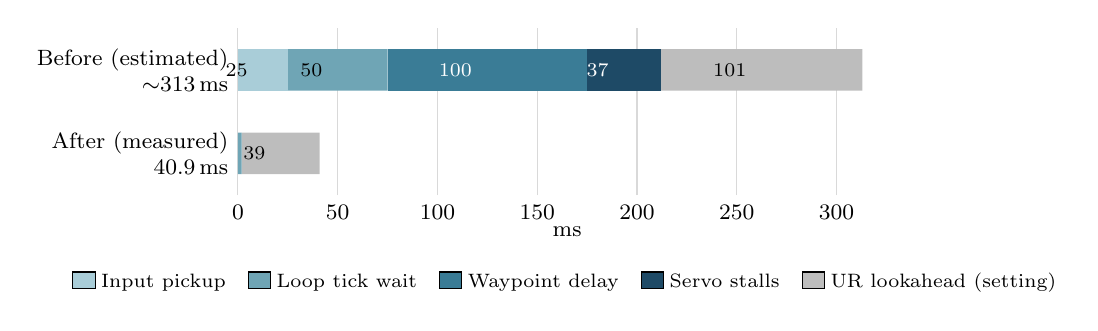
\begin{tikzpicture}
\begin{axis}[
    xbar stacked,
    width=0.82\linewidth, height=3.7cm,
    xmin=0, xmax=330,
    xlabel={ms}, xlabel style={font=\footnotesize, yshift=4pt},
    tick label style={font=\footnotesize},
    symbolic y coords={After, Before},
    ytick={After, Before},
    yticklabels={After (measured)\\40.9\,ms, Before (estimated)\\$\sim$313\,ms},
    yticklabel style={align=right, font=\footnotesize},
    enlarge y limits=0.5,
    bar width=15pt,
    axis line style={draw=none}, tick style={draw=none},
    xmajorgrids, grid style={gray!30},
    nodes near coords={\pgfmathfloattofixed{\pgfplotspointmeta}\pgfmathtruncatemacro{\v}{\pgfmathresult}\ifnum\v<12\else\v\fi},
    nodes near coords style={font=\scriptsize, anchor=east, xshift=-2pt, text=black},
    point meta=rawx,
    legend style={at={(0.5,-0.40)}, anchor=north, legend columns=-1, font=\scriptsize, draw=none,
                  /tikz/every even column/.append style={column sep=6pt}},
    legend cell align=left,
]
\addplot[fill=latA, draw=none] coordinates {(25,Before) (0,After)};
\addplot[fill=latB, draw=none] coordinates {(50,Before) (1.9,After)};
\addplot[fill=latC, draw=none, nodes near coords style={text=white}] coordinates {(100,Before) (0,After)};
\addplot[fill=latD, draw=none, nodes near coords style={text=white}] coordinates {(37,Before) (0,After)};
\addplot[fill=latE, draw=none] coordinates {(101,Before) (39,After)};
\legend{Input pickup, Loop tick wait, Waypoint delay, Servo stalls, UR lookahead (setting)}
\end{axis}
\end{tikzpicture}
\caption{Hand-to-arm latency in ms, old code estimated and new code measured.}
\label{fig:latency}
\end{figure}

\section{Force Sensor Fault Resolved}

The periodic force excursions reported to MAE were a grounding problem, not a sensor fault: the interface box now
takes USB power from a grounded HP USB-C Dock G5, and the white grounding wire is insulated, so the sensor sees one
ground reference instead of two (wall plug and metal table).
Since October~14 the rest readings on the plots stay within $\pm 0.1$\,N, which is sufficient for our accuracy
requirement.

\section{Admittance Control with Geoffrey}

Geoffrey's admittance controller was reviewed and merged on October~14; I made a few improvements (see 
\href{https://gitlabc.nrc-cnrc.gc.ca/Yiran.Liu/nrc_robot_manipulation/-/blob/teleop-refactor/Documentation/Journal/2026Oct/AdmittanceControllerReview.md}{\texttt{AdmittanceControllerReview.md}}).
The severe lagginess he experienced while testing was due to the laggacy loop: it ran at <50\,Hz and dropped 86\,\% of the sensor's packets.
I ported the controller to the new codebase, the demo runs smoothly under the 500\,Hz loop. This opens rotation compliance and force feedback and next steps for Geoffrey.

\section{Force Feedback Proposal}
\label{sec:ff}

I drafted \emph{Force Feedback Refinement} (October~8), shared with the team on Overleaf.
It separates contact force from the sensor's inertial and gravity terms, states the baseline, and proposes an
admittance model whose spring force is what the operator feels, an asynchronous split (Figure~\ref{fig:async}) in
which the robot sends a contact model at low rate and the Haply renders it at kHz rate, which the refactored
runtime already reserves, and sensor calibration by system identification. Experiments remain to be planned.

\begin{figure}[H]
\centering
\resizebox{0.74\linewidth}{!}{%
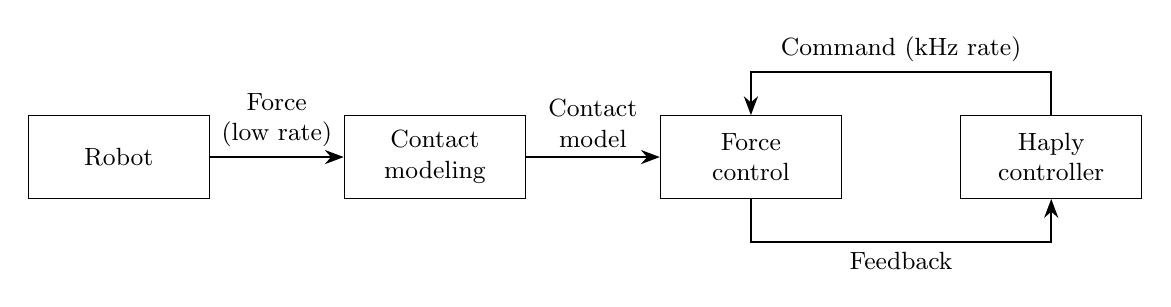
\begin{tikzpicture}[
    box/.style={draw, rectangle, minimum width=2.3cm, minimum height=1.05cm, align=center, font=\small},
    arr/.style={-{Stealth[length=2.4mm]}, semithick},
    lab/.style={font=\small, align=center},
]
\node[box] (robot) {Robot};
\node[box, right=1.7cm of robot] (model) {Contact\\modeling};
\node[box, right=1.7cm of model] (fc) {Force\\control};
\node[box, right=1.5cm of fc] (haply) {Haply\\controller};
\draw[arr] (robot) -- node[lab, above] {Force\\(low rate)} (model);
\draw[arr] (model) -- node[lab, above] {Contact\\model} (fc);
\draw[arr] (haply.north) -- ++(0,0.55) coordinate (c) -- (c -| fc.north) node[lab, midway, above] {Command (kHz rate)} -- (fc.north);
\draw[arr] (fc.south) -- ++(0,-0.55) coordinate (f) -- (f -| haply.south) node[lab, midway, below] {Feedback} -- (haply.south);
\end{tikzpicture}}
\caption{The asynchronous feedback loop.}
\label{fig:async}
\end{figure}

\section{Temporary Fix for the Old Training Code}

The normalizer was fit on absolute poses while the model trains on poses relative to the start pose; with rotation
frozen in teleop, normalized rotation targets sat near $-14\,000$ and the press dataset did not train.
The fix on \texttt{main} (October~16, \href{https://gitlabc.nrc-cnrc.gc.ca/Yiran.Liu/nrc_robot_manipulation/-/blob/teleop-refactor/Training/dataset/relative_dataset.py}{\texttt{relative\_dataset.py}}) fits it on the relative poses, so
every sample lies in $[-1, 1]$.
The MSE now converges on the dataset Linda and Geoffrey collected, and inference runs.
% The commit names the datasets test_press and lamp_50; confirm the dataset name above.

\section{Policy Refactor Plan and Dashboard}
\label{sec:policy}

The plan is shared on Teams as an editable document and kept in
\href{https://gitlabc.nrc-cnrc.gc.ca/Yiran.Liu/nrc_robot_manipulation/-/blob/teleop-refactor/Documentation/Journal/2026Oct/PolicyRefactor.md}{\texttt{PolicyRefactor.md}}, with the technical details in
\href{https://gitlabc.nrc-cnrc.gc.ca/Yiran.Liu/nrc_robot_manipulation/-/blob/teleop-refactor/Documentation/Journal/2026Oct/PolicyRefactorExecutionJournal.md}{\texttt{PolicyRefactorExecutionJournal.md}}:
LeRobot for training and models, our own runtime above it and our models as a plugin below it.
Following your feedback at Wednesday's meeting, that we need a way to verify dataset quality and policy output
correctness, I specified and prototyped a dashboard (Figure~\ref{fig:dash}) to visualize the full details of the robot in operation. This dashboard runs live during teleop and policy rollout to make behavior transparent; it also provide collected data playback for dataset inspection 
(\href{https://gitlabc.nrc-cnrc.gc.ca/Yiran.Liu/nrc_robot_manipulation/-/blob/teleop-refactor/src/shared/inspect_log.py}{\texttt{inspect\_log.py}}). 
Implemented using Rerun.

\begin{figure}[H]
\centering
\begin{minipage}[c]{0.6\linewidth}
\centering
% Source: Documentation/Journal/2026Oct/Dashboard.png
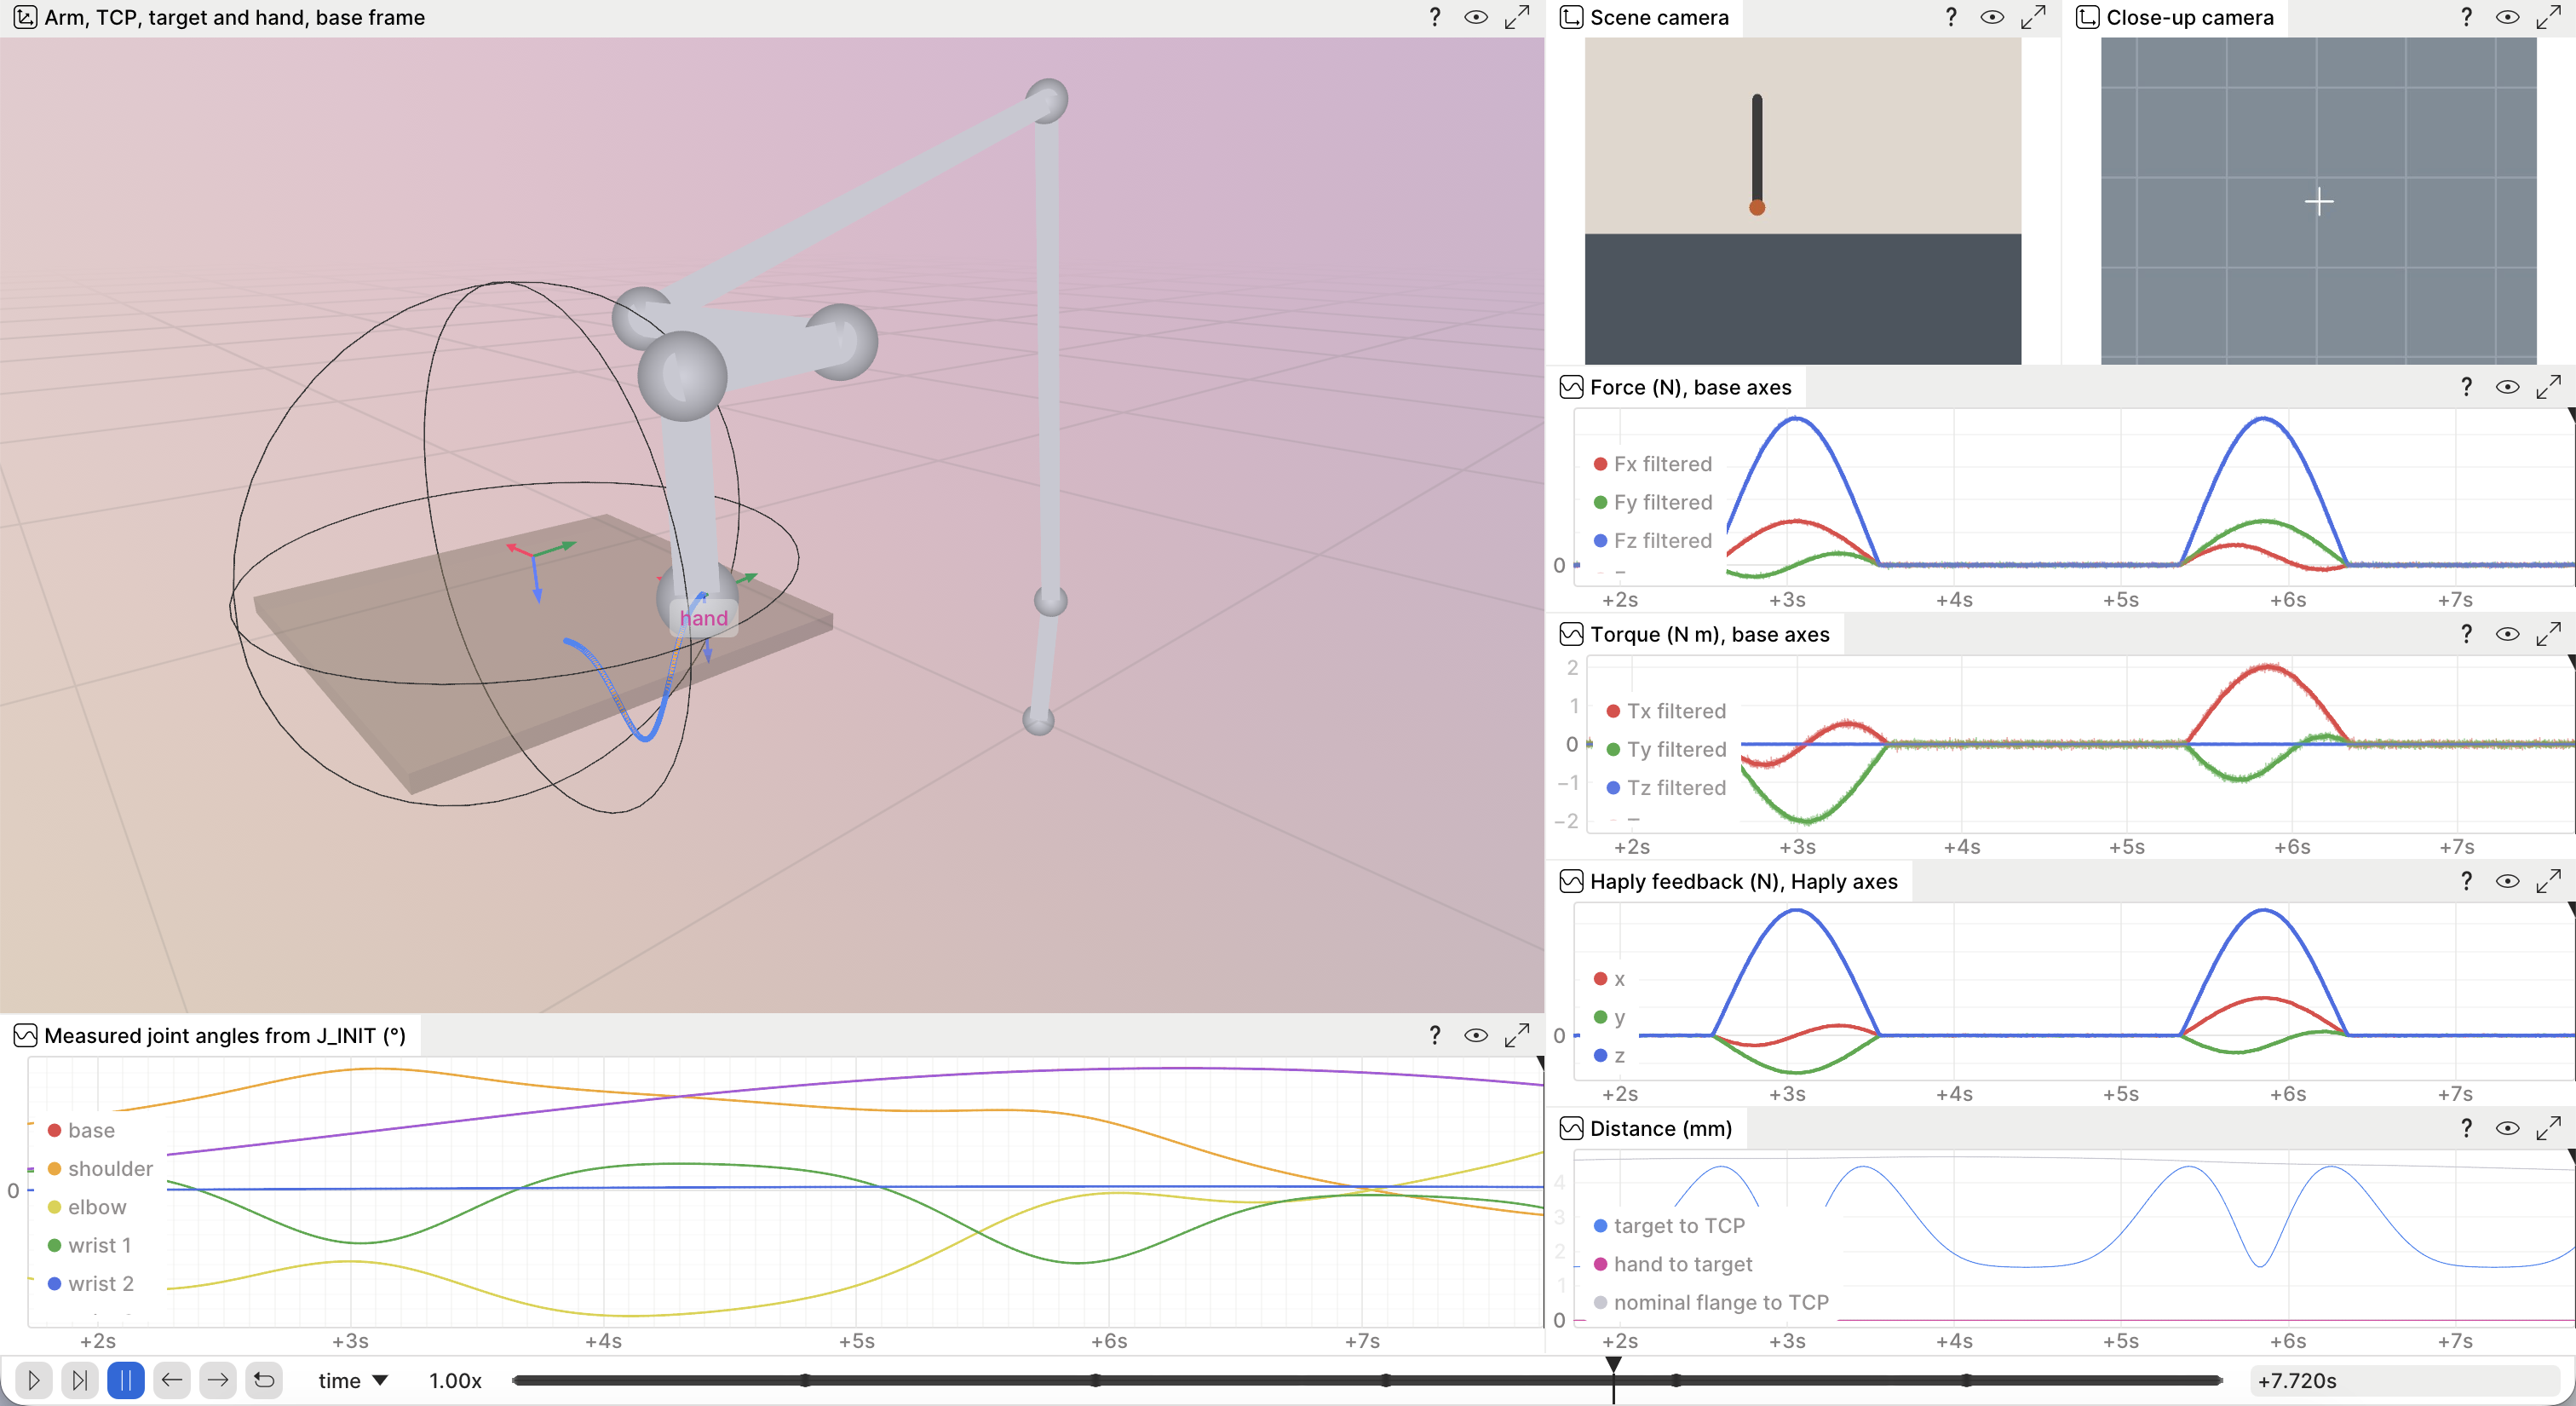
\includegraphics[width=\linewidth]{./Dashboard.png}
\end{minipage}\hspace{0.03\linewidth}%
\begin{minipage}[c]{0.3\linewidth}
\caption{The dashboard prototype showing measured robot joints, measured end-effector pose, end-effector trajectory, operator command, camera views, and force measurement.}
\label{fig:dash}
\end{minipage}
\end{figure}

\section{Plan for Next Week}

\begin{enumerate}
    \item \textbf{Teleoperation refactor.} Validate Stage~3 on hardware, implement Stage~4 and rehearse a collection
    run; This will allow Linda to start collecting data with the refactored and fully functional teleop code.
    \item \textbf{Policy refactor.} Set up the LeRobot environment and dataset converter;
    train LeRobot's diffusion policy on the legacy press data and confirm its convergence on our data; Measure trajectory MSE, and visually inspect trajectory output on frozen frames. 
    classes.
    \item \textbf{Shadow mode, if the above lands.} The policy predicts from live sensors and cameras while the
    operator teleoperates, with its chunks shown on the dashboard; nothing is executed.
    \item \textbf{Force feedback.} Discuss the force feedback command interface design with Geoffrey so he can start exploring.
\end{enumerate}

% \section{Currently Waiting On}
% TODO: KIMM: initial meeting and proposal status, if there is something to wait on.

\medskip\noindent\textbf{Other projects.}
Collaboration with Dr.~Shu's human motion project and Shunyu's work are paused,
since you requested that I prioritized the robotics project. The refactor has taken all of my time, and neither of them asked
for help on any specific item.

\end{document}
